\section{Data preprocessing} \label{sec:dataset_creation} % ----------------------------------------------------+

\begin{figure}[ht!]
    \centering
        \subfloat[KTH]{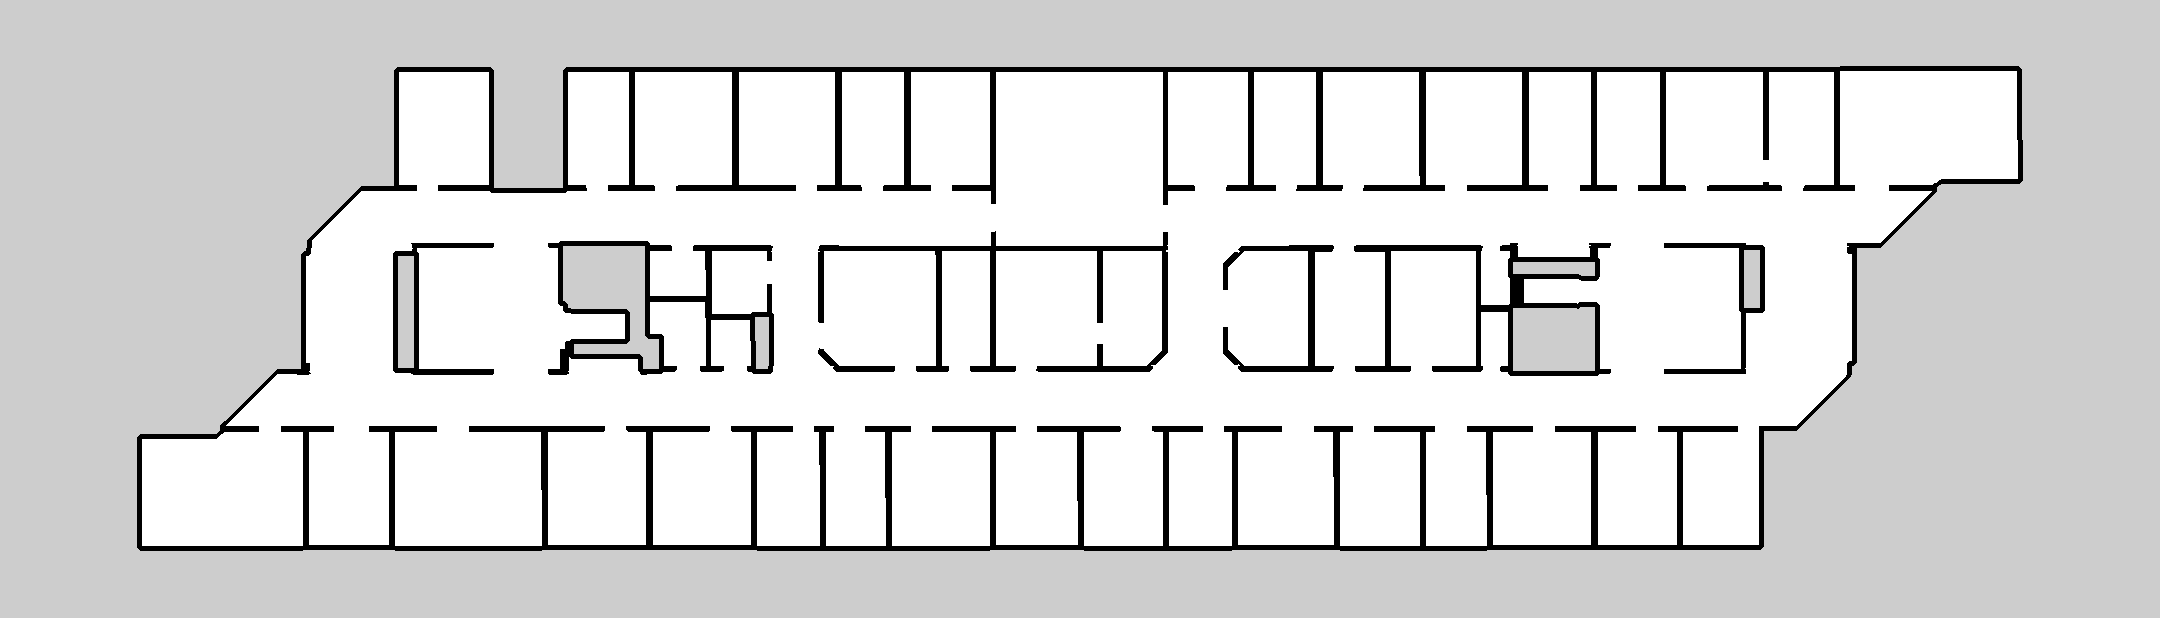
\includegraphics[width=.3\linewidth, angle=90]{images/50041171.png}}\hspace{.3in}
        \subfloat[MIT]{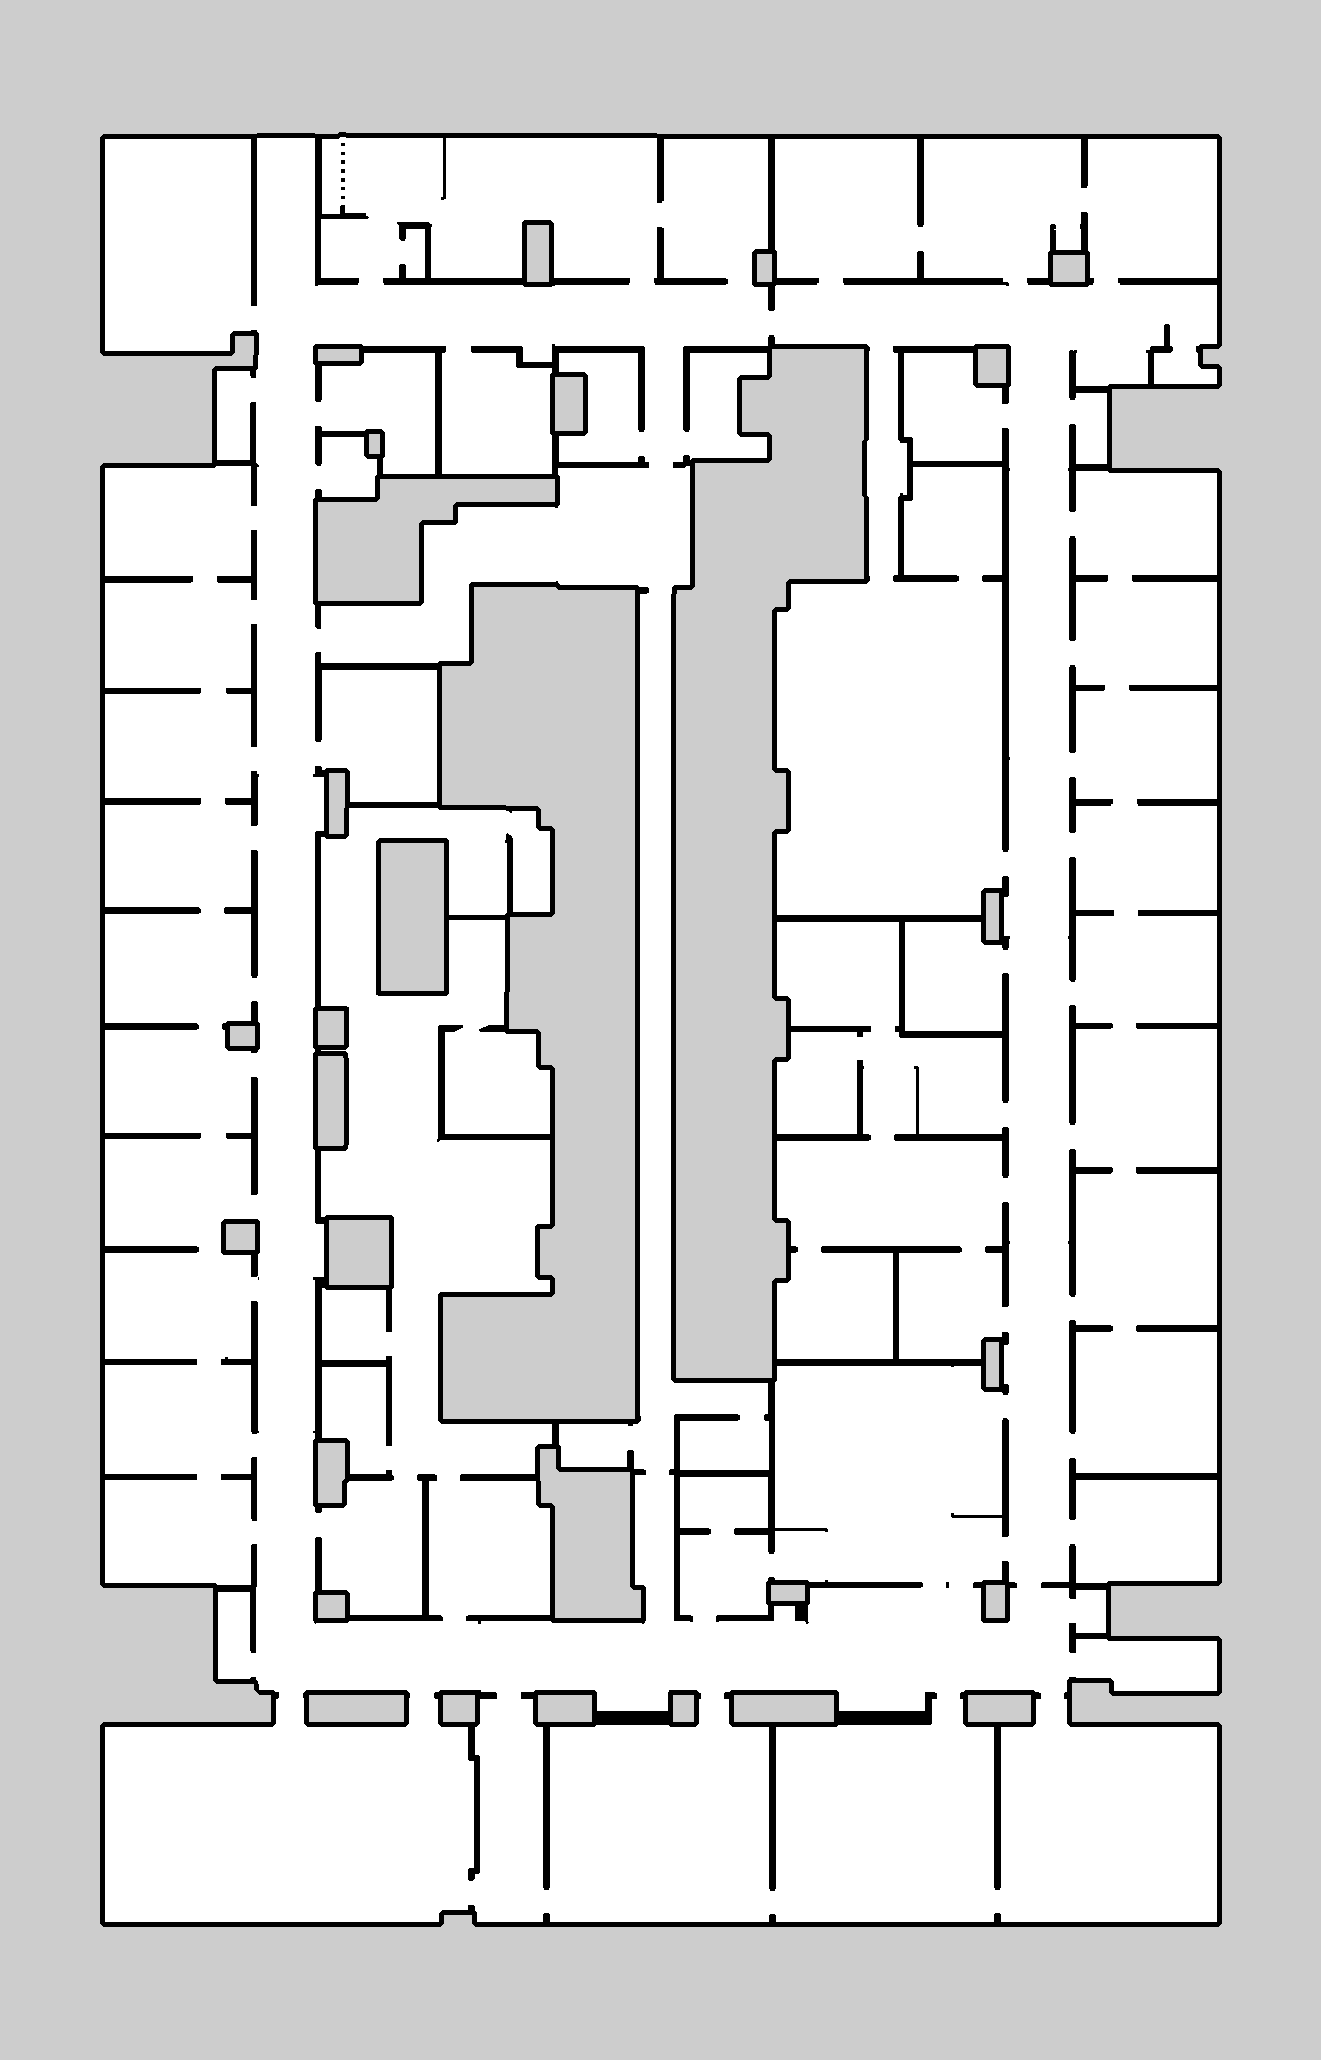
\includegraphics[height=.3\linewidth]{images/12-1.png}}\hspace{.3in}
        \subfloat[HouseExpo]{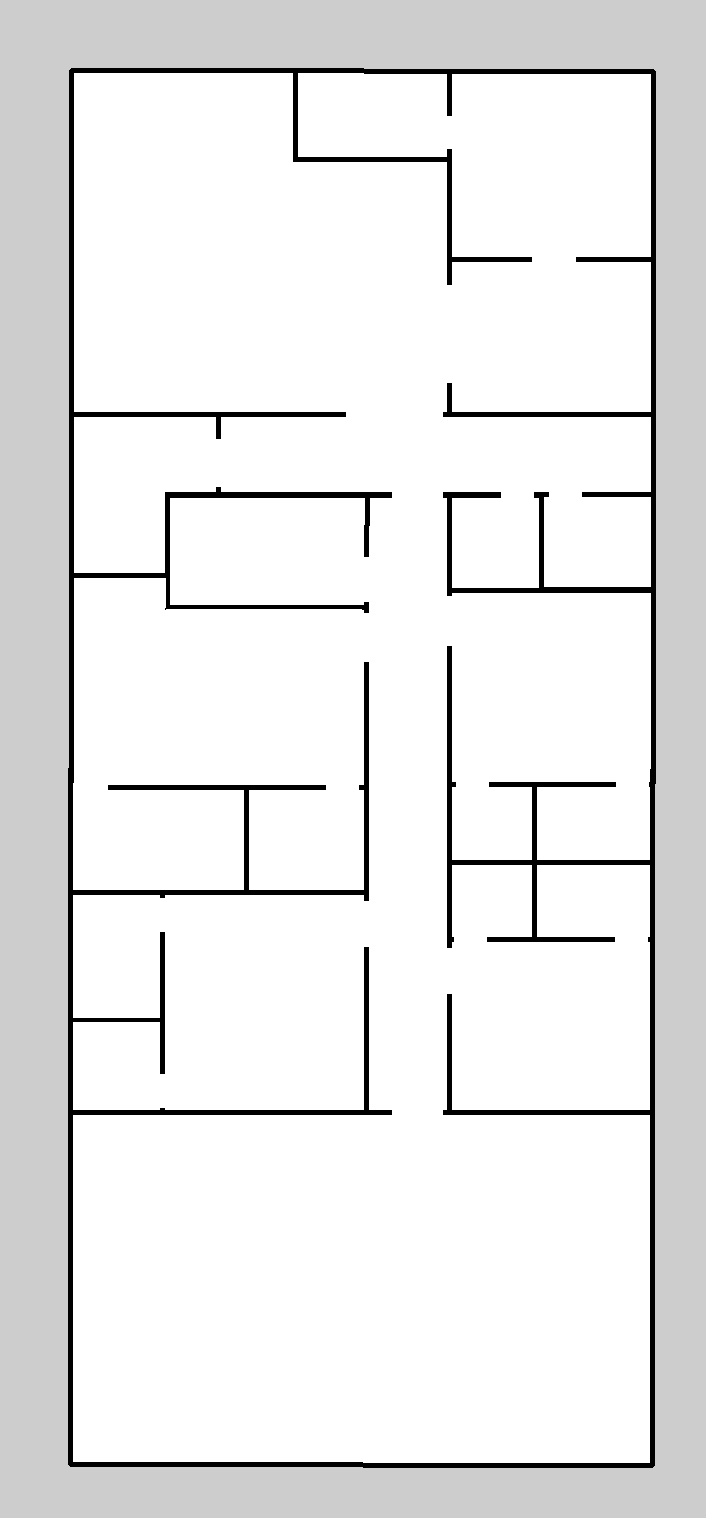
\includegraphics[height=.3\linewidth]{images/0a47882b40daf033e05e0b2dffafa6f7.png}}
    \caption{Example of floorplans from the datasets used in this work.}\label{fig:maxExample}
\end{figure}

\noindent
The dataset used in this work  consists of floorplans and exploration data from three different sources: MIT campus \cite{whiting2006geometric}, KTH campus \cite{aydemir2012KTH}, and HouseExpo \cite{li2019houseexpo}. 
The joint dataset consists of 5933 floorplans, and contains both domestic and work, school environments, as shown in \textbf{Figure \ref{fig:maxExample}}.\\

\begin{figure}[ht!]
    \centering
        \subfloat{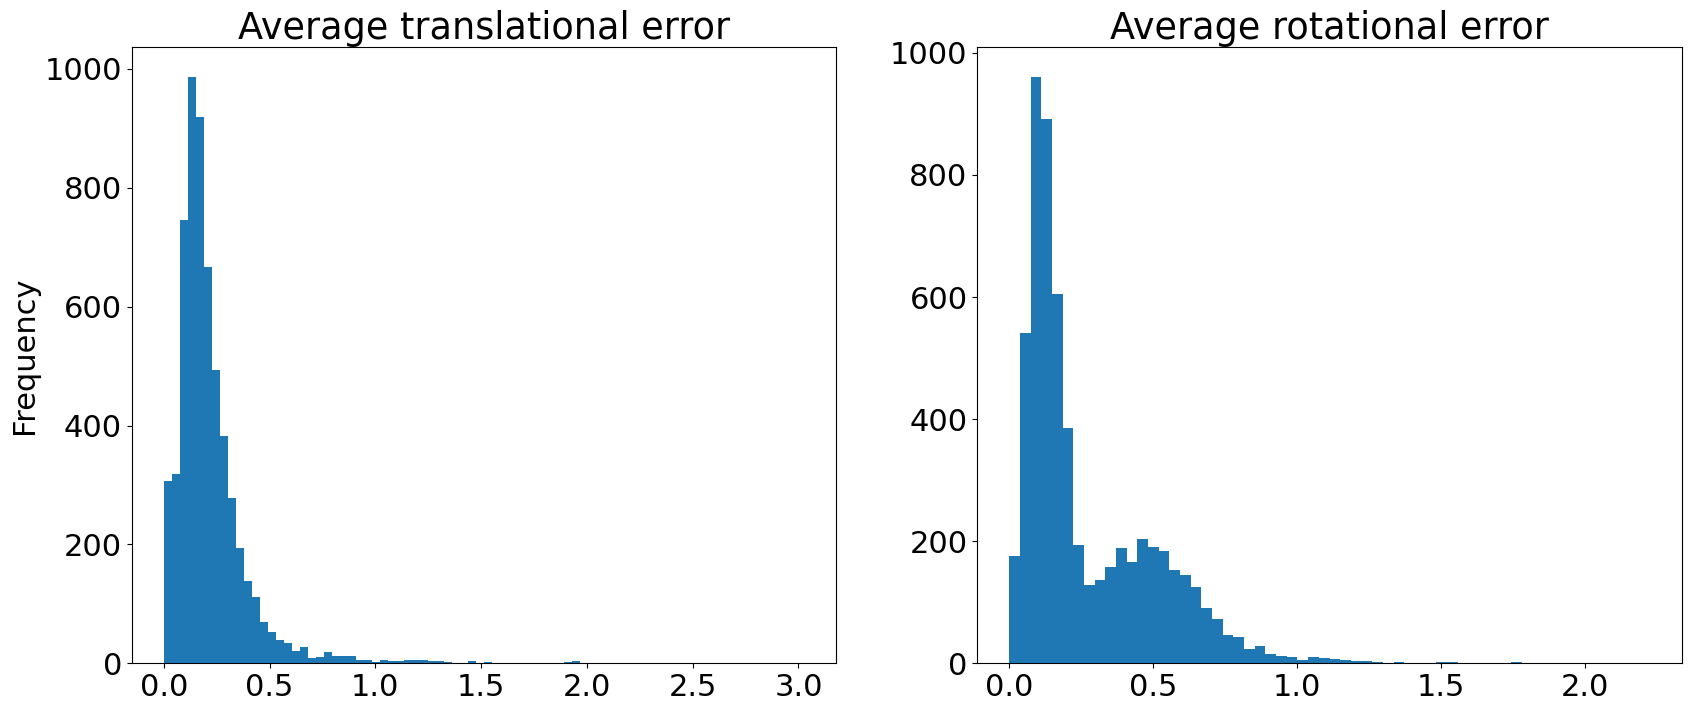
\includegraphics[width=.8\linewidth]{images/data_distribution.png}}
    \caption{Original localization error distribution}\label{fig:dataDistribution}
\end{figure}

\begin{figure}[ht!]
    \centering
        \subfloat{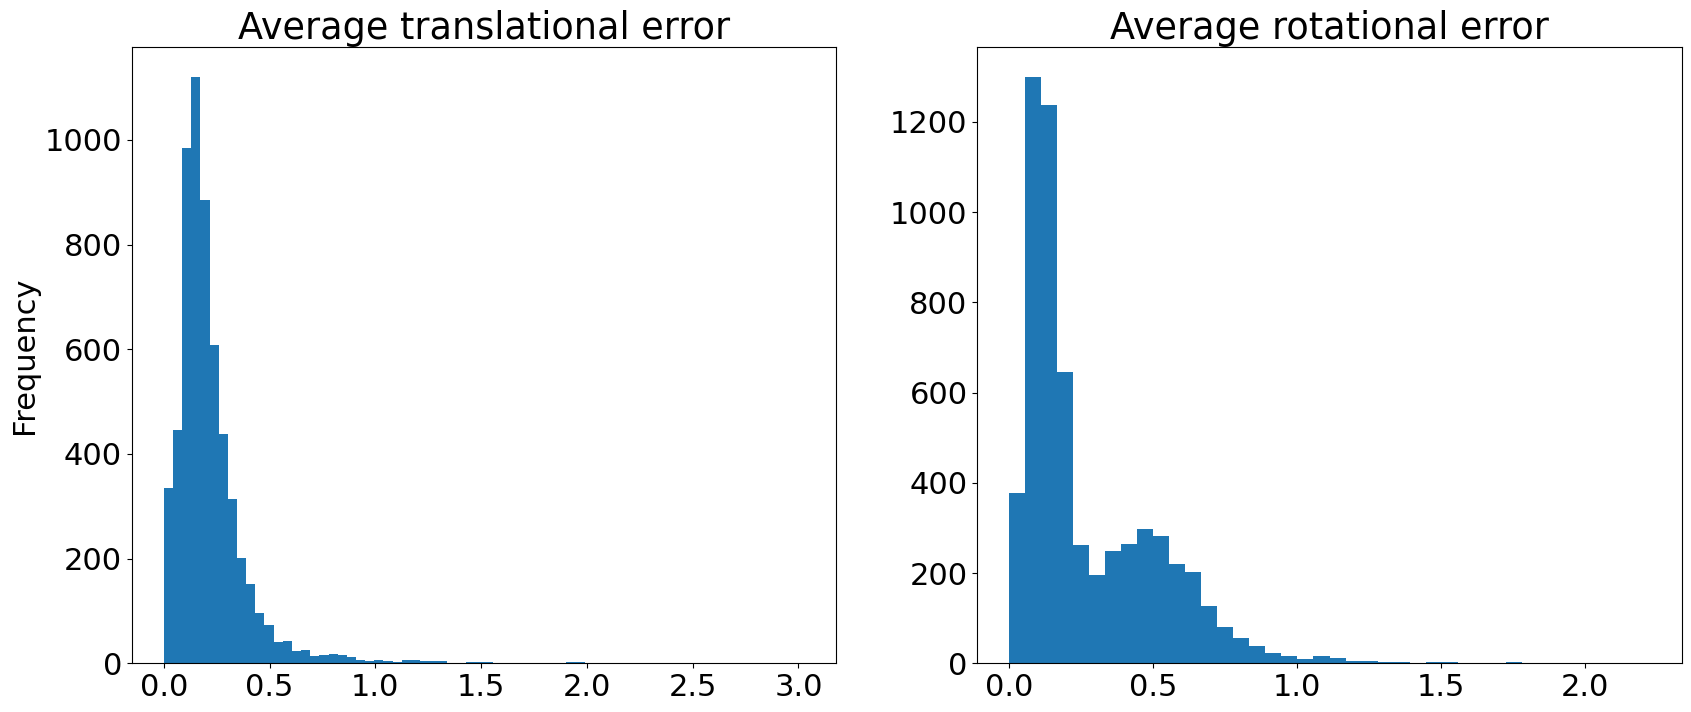
\includegraphics[width=.8\linewidth]{images/scaled_data.png}}
    \caption{Re-scaled localization errors}\label{fig:dataDistribution_scaled}
\end{figure}

\noindent
The first step consists in visualizing the distribution of the data in our dataset, as shown in \textbf{Figure \ref{fig:dataDistribution}}, where we observe that the ATE and ARE distributions are respectively unimodal and bimodal, both with a short right tail and a small number of outliers.

The two quantities we want to estimate are distributed on distinct ranges and, to ensure that our models learn to predict each quantity proportionately, the data has to be re-scaled so that 99\% of the values fall between 0 and 1, as shown in \textbf{Figure \ref{fig:dataDistribution_scaled}}. Additionally, the area of each floorplan is normalized as well to the $[0, 1]$ interval by dividing each datapoint by the maximum area value in the dataset.

% -----------------------------------------------------------
%                                                           \
%                                                           \
% -----------------------------------------------------------

%\subsection{Image loading and dataset creation}\label{sec:dataset_creation} % ---------------------------------------
\noindent
Another preprocessing step consists in fixing images' resolution so that they can be fed to the CNN: for each floorplan we compute the minimum squared bounding box and scale it to a size \footnote{This resolution choice is rather generous, given that both CNNs internally re-scale the image to 224x224px. Storing the dataset at a higher resolution leaves some margin for future experiments with different models.} of 500x500px. 
Floorplan images are loaded and processed lazily using TensorFlow's \texttt{data} API\footnote{https://www.tensorflow.org/guide/data}, which automatically handles the allocation and de-allocation policies for the images. 

After splitting the floorplans in the usual train/validation/test partitions, respectively with 70/15/15 thresholds, the dataset creation steps consist of:
\begin{enumerate}
    \item Image loading.
    \item Data augmentation, which randomly rotates an image by multiples of 90°.
    \item Creation of each datapoint tuple \texttt{(image, area, label)}.
    \item Shuffling and batching of datapoints into mini-batches of size 64.
\end{enumerate}
Note that the data augmentation step is applied at runtime only on the training set, in order to improve the model generalization capabilities. 

The vast majority of environments in the dataset satisfy the \textit{Manhattan World} assumption, which states that all of the walls of an environment are aligned to two main directions, orthogonal to each other. Moreover, the main directions of the floorplan images are aligned with the image borders (i.e.,  most walls are either horizontal or vertical), thus, the choice of using multiples of 90° for image augmentation, is made to preserve the alignment of the walls.

